 \section{Cerința problemei}
\subsection{Intersectie nedirijata}
Avem patru mașini într-o intersecție nedirijată: M1, M2, M3, M4.
\newline
Intersecția e bazată pe desenul din cerință.
\newline
Cele două străzi sunt cu dublu sens.
\newline
 \begin{itemize}
    \setlength\itemsep{0em}
    \item M1 nu semnalizează și merge în față.
    \item M2 semnalizează dreapta.
    \item M3 semnalizează stânga.
    \item M4 nu semnalizează și merge în față.

\end{itemize}


M1 se află în dreapta lui M4, M2 se află în dreapta lui M1, M3 se afla în dreapta lui M2, M4 se află în dreapta lui M3.

Vrem să determinăm dacă trece M2 primul, M1 al doilea, M4 al treilea și M3 ultimul.


\begin{figure}[htb]
  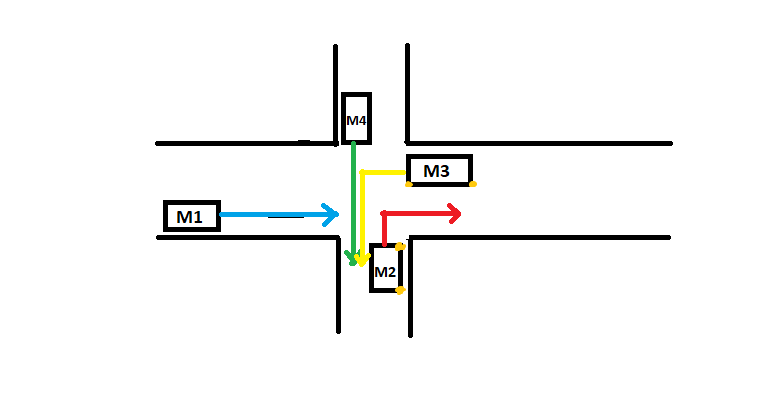
\includegraphics[width=\linewidth]{car.png}
 \caption{Intersectia nedirijata.}
  \label{fig:boat1}
  \end{figure}


\newpage

\subsection{Intersectie dirijata}

Avem patru mașini într-o intersecție dirijată: M1, M2, M3, M4.
\newline
Intersecția e bazată pe desenul din cerință.
\newline
Cele două străzi sunt cu dublu sens.
\newline

\newline
 \begin{itemize}
    \setlength\itemsep{0em}
    \item M1 semnalizează stânga și se află pe strada cu semnul CEDEAZĂ.
    \item M2 nu semnalizează și merge în față și se află pe strada cu prioritate.
    \item M3  nu semnalizează și merge în față și se află pe strada cu semnul STOP.
    \item M4  semnalizează stânga și se află pe strada cu prioritate.

\end{itemize}

Vrem să determinăm dacă trece M2 primul, M4 al doilea, M3 al treilea și M1 ultimul.

\begin{figure}[htb]
  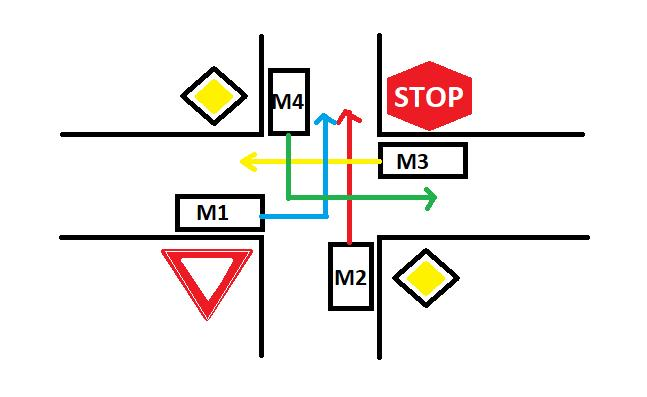
\includegraphics[width=\linewidth]{car2.jpg}
 \caption{Intersectia dirijata.}
  \label{fig:boat1}
  \end{figure}
